\documentclass[a4paper,12pt]{article}

\usepackage[utf8x]{inputenc}
\usepackage[T2A]{fontenc}
\usepackage[english, russian]{babel}

% Опционно, требует  apt-get install scalable-cyrfonts.*
% и удаления одной строчки в cyrtimes.sty
% Сточку не удалять!
% \usepackage{cyrtimes}

% Картнки и tikz
\usepackage{graphicx}
\usepackage{tikz}
\usetikzlibrary{snakes,arrows,shapes}


% Некоторая русификация.
\usepackage{misccorr}
\usepackage{indentfirst}
\renewcommand{\labelitemi}{\normalfont\bfseries{--}}

% Увы, поля придётся уменьшить из-за листингов.
\topmargin -1cm
\oddsidemargin -0.5cm
\evensidemargin -0.5cm
\textwidth 17cm
\textheight 24cm

\sloppy

% Оглавление в PDF
\usepackage[
bookmarks=true,
colorlinks=true, linkcolor=black, anchorcolor=black, citecolor=black, menucolor=black,filecolor=black, urlcolor=black,
unicode=true
]{hyperref}

% Для исходного кода в тексте
\newcommand{\Code}[1]{\texttt{#1}}

\usepackage{verbatim}
\usepackage{fancyvrb}
\fvset{frame=leftline, fontsize=\small, framerule=0.4mm, rulecolor=\color{darkgray}, commandchars=\\\{\}}
\renewcommand{\theFancyVerbLine}{\small\arabic{FancyVerbLine}}


\title{Отчёт по лабораторной работе \\ <<Динамическая IP-маршрутизация>>}
\author{Trung Luong}

\begin{document}

\maketitle

\tableofcontents

\section{Настройка сети}

\subsection{Топология сети}

Топология сети и используемые IP-адреса показаны на рисунке~\ref{fig:network}.

\begin{figure}
\centering
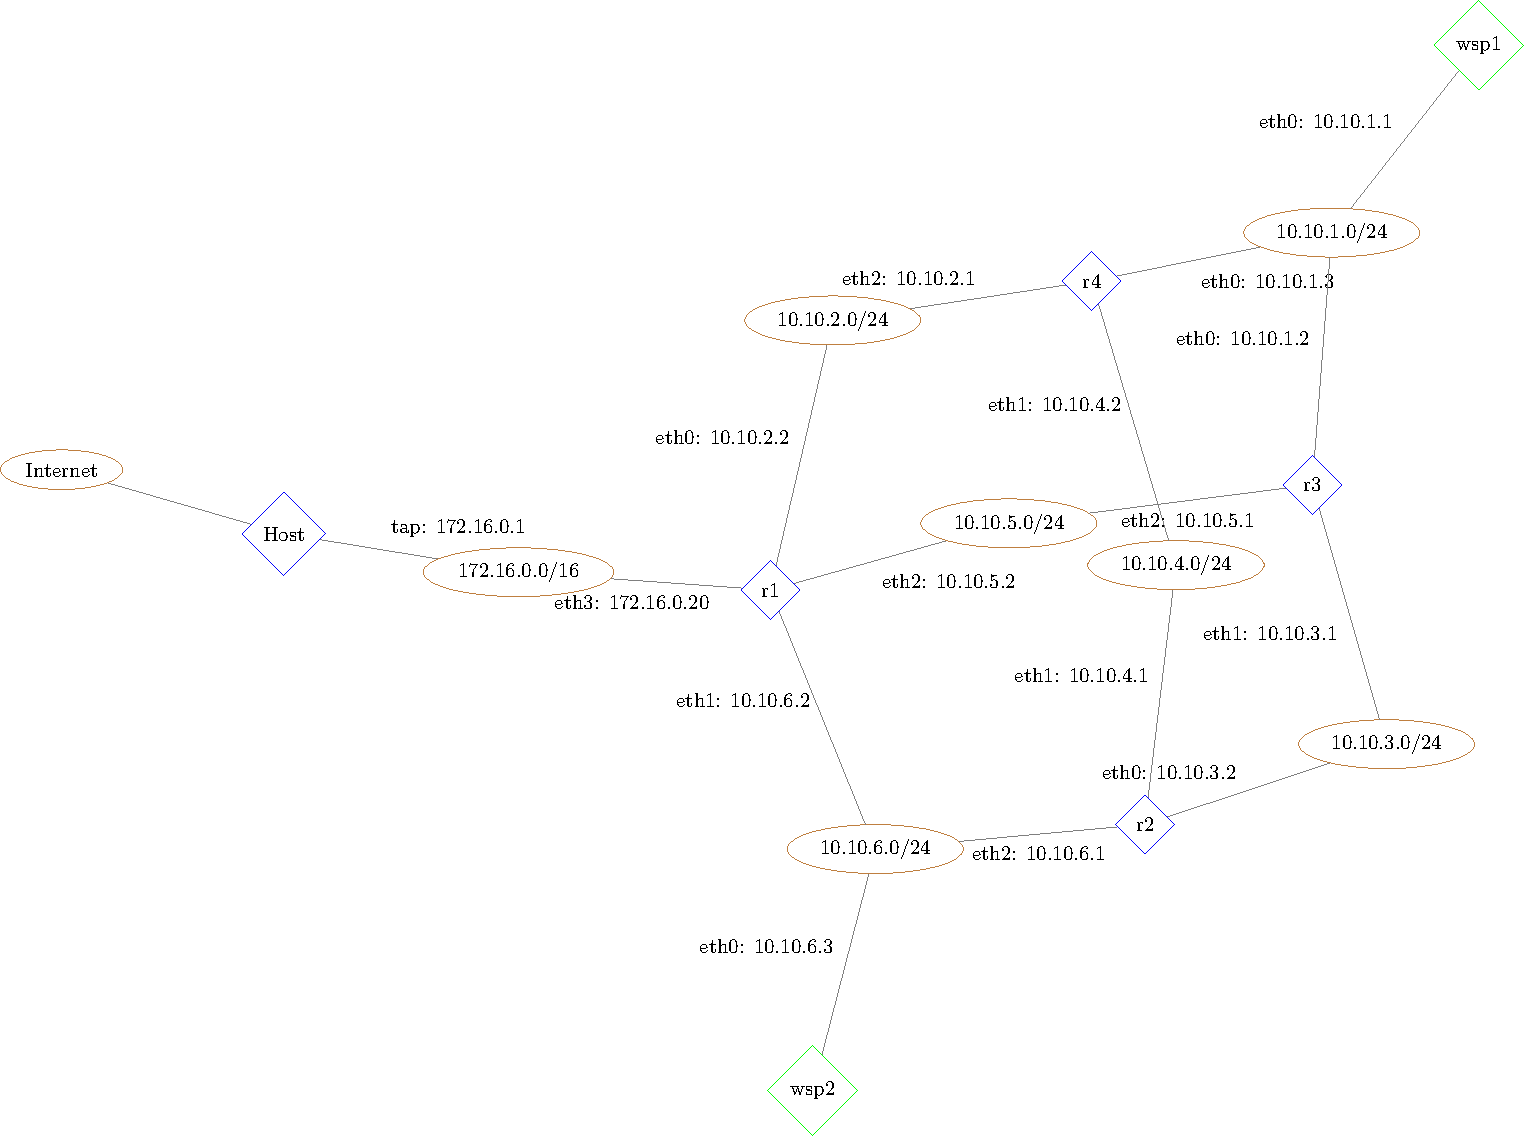
\includegraphics[width=0.8\textwidth]{includes/network_gv.pdf}
\caption{Топология сети}
\label{fig:network}
\end{figure}

Перечень узлов, на которых используется динамическая IP-маршрутизация: все


\subsection{Назначение IP-адресов}

Ниже приведён файл сетевой настройки  маршрутизатора \textbf{r1}.

\begin{Verbatim}
auto lo
iface lo inet loopback

auto eth0
iface eth0 inet static
address 10.10.2.2
netmask 255.255.255.0

auto eth1
iface eth1 inet static
address 10.10.6.2
netmask 255.255.255.0

auto eth2
iface eth2 inet static
address 10.10.5.2
netmask 255.255.255.0
\end{Verbatim}

Ниже приведён файл сетевой настройки рабочей станции \textbf{wsp1}.

\begin{Verbatim}
auto lo
iface lo inet loopback

auto eth0
iface eth0 inet static
address 10.10.1.1
netmask 255.255.255.0
\end{Verbatim}


\subsection{Настройка протокола RIP}

Ниже приведен файл \Code{/etc/quagga/ripd.conf} маршрутизатора \textbf{r1}.

\begin{Verbatim}
! Этот настройки, касающиеся протокола RIP.
router rip

! Раскомментируйте ниже все интерфейсы, подключённые
! к сетям с другими маршрутизаторами.
network eth0
network eth1
network eth2
! network eth3

! Уменьшаем значения всех таймеров для ускорения опытов.
! Рассылка: 10 сек., устаревание: 60 cек., сборка мусора: 120 сек.
timers basic 10 60 120

! Следующие две строчки заставляют маршрутизатор
! добавлять в сообщения протокола RIP все известные ему маршруты.
redistribute kernel
! redistribute connected

! Это имя файла журнала службы RIP.
! Его содержимое можно изучить в случае неполадок
log file /var/log/quagga/ripd.log
\end{Verbatim}


Ниже приведен файл \Code{/etc/quagga/ripd.conf} рабочий станции, связанной с несколькими маршрутизаторами \textbf{wsp1}.

\begin{Verbatim}
! Этот настройки, касающиеся протокола RIP.
router rip

! Раскомментируйте ниже все интерфейсы, подключённые
! к сетям с другими маршрутизаторами.
network eth0
! network eth1
! network eth2

! Уменьшаем значения всех таймеров для ускорения опытов.
! Рассылка: 10 сек., устаревание: 60 cек., сборка мусора: 120 сек.
timers basic 10 60 120

! Следующие две строчки заставляют маршрутизатор
! добавлять в сообщения протокола RIP все известные ему маршруты.
redistribute kernel
redistribute connected

! Это имя файла журнала службы RIP.
! Его содержимое можно изучить в случае неполадок
log file /var/log/quagga/ripd.log
\end{Verbatim}


\section{Проверка настройки протокола RIP}

Вывод \textbf{traceroute} от узла \textbf{wsp2} до \textbf{wsp1} при нормальной работе сети.

\begin{Verbatim}
wsp2:~# traceroute -n 10.10.1.1
traceroute to 10.10.1.1 (10.10.1.1), 64 hops max, 40 byte packets
 1  10.10.6.1  1 ms  0 ms  0 ms
 2  10.10.3.1  11 ms  0 ms  0 ms
 3  10.10.1.1  25 ms  0 ms  1 ms
\end{Verbatim}

Вывод \textbf{traceroute} от узла такого-то до внешнего IP (195.19.38.2 сгодится).

\begin{Verbatim}
Сюда нужно поместить вывод traceroute.
\end{Verbatim}

Вывод сообщения RIP.

\begin{Verbatim}
r2:~# tcpdump -tvn -s 1518 udp -i eth0
tcpdump: listening on eth0, link-type EN10MB (Ethernet), capture size 1518 bytes
IP (tos 0x0, ttl 1, id 0, offset 0, flags [DF], proto UDP (17), length 92) 10.10.3.2.520 > 224.0.0.9.520: 
	RIPv2, Response, length: 64, routes: 3
	  AFI: IPv4:       10.10.2.0/24, tag 0x0000, metric: 2, next-hop: self
	  AFI: IPv4:       10.10.4.0/24, tag 0x0000, metric: 1, next-hop: self
	  AFI: IPv4:       10.10.6.0/24, tag 0x0000, metric: 1, next-hop: self
IP (tos 0x0, ttl 1, id 0, offset 0, flags [DF], proto UDP (17), length 112) 10.10.3.1.520 > 224.0.0.9.520: 
	RIPv2, Response, length: 84, routes: 4
	  AFI: IPv4:       10.10.1.0/24, tag 0x0000, metric: 1, next-hop: self
	  AFI: IPv4:       10.10.2.0/24, tag 0x0000, metric: 2, next-hop: self
	  AFI: IPv4:       10.10.4.0/24, tag 0x0000, metric: 2, next-hop: self
	  AFI: IPv4:       10.10.5.0/24, tag 0x0000, metric: 1, next-hop: self
...
\end{Verbatim}

Вывод таблицы RIP.

\begin{Verbatim}
r1# show ip rip
Codes: R - RIP, C - connected, S - Static, O - OSPF, B - BGP
Sub-codes:
      (n) - normal, (s) - static, (d) - default, (r) - redistribute,
      (i) - interface

     Network            Next Hop         Metric From            Tag Time
R(n) 10.10.1.0/24       10.10.2.1             2 10.10.2.1         0 00:52
C(i) 10.10.2.0/24       0.0.0.0               1 self              0
R(n) 10.10.3.0/24       10.10.5.1             2 10.10.5.1         0 00:52
R(n) 10.10.4.0/24       10.10.2.1             2 10.10.2.1         0 00:52
C(i) 10.10.5.0/24       0.0.0.0               1 self              0
C(i) 10.10.6.0/24       0.0.0.0               1 self              0
\end{Verbatim}

Вывод таблицы маршрутизации.

\begin{Verbatim}
r1:~# ip r
10.10.6.0/24 dev eth1  proto kernel  scope link  src 10.10.6.2 
10.10.4.0/24 via 10.10.2.1 dev eth0  proto zebra  metric 2 
10.10.5.0/24 dev eth2  proto kernel  scope link  src 10.10.5.2 
10.10.2.0/24 dev eth0  proto kernel  scope link  src 10.10.2.2 
10.10.3.0/24 via 10.10.5.1 dev eth2  proto zebra  metric 2 
10.10.1.0/24 via 10.10.2.1 dev eth0  proto zebra  metric 2 
172.16.0.0/16 dev eth3  proto kernel  scope link  src 172.16.0.20 
default via 172.16.0.1 dev eth3 
\end{Verbatim}


\section{Расщепленный горизонт и испорченные обратные обновления}

Поместить сюда вывод сообщения одного и того же маршрутизатор с включенным расщ. горизонтом, с включенными испорченными обновлениями, с отключённым расщ. гор.

\begin{Verbatim}
# r4/etc/quagga/ripd.conf
interface eth0
ip rip split-horizon poisoned-reverse

# bash
r4:~# tcpdump -tnv udp -i eth0
tcpdump: listening on eth0, link-type EN10MB (Ethernet), capture size 96 bytes
IP (tos 0x0, ttl 1, id 0, offset 0, flags [DF], proto UDP (17), length 172) 10.10.1.3.520 > 224.0.0.9.520: 
	RIPv2, Response, length: 144, routes: 7
	  AFI: IPv4:         0.0.0.0/0 , tag 0x0000, metric: 2, next-hop: self
	  AFI: IPv4:       10.10.1.0/24, tag 0x0000, metric: 16, next-hop: self[|rip]
IP (tos 0x0, ttl 1, id 0, offset 0, flags [DF], proto UDP (17), length 112) 10.10.1.2.520 > 224.0.0.9.520: 
	RIPv2, Response, length: 84, routes: 4
	  AFI: IPv4:         0.0.0.0/0 , tag 0x0000, metric: 2, next-hop: self
	  AFI: IPv4:       10.10.3.0/24, tag 0x0000, metric: 1, next-hop: self[|rip]
...
\end{Verbatim}

\begin{Verbatim}
# r4/etc/quagga/ripd.conf
interface eth0
no ip rip split-horizon

# bash
r4:~# tcpdump -tnv udp -i eth0
tcpdump: listening on eth0, link-type EN10MB (Ethernet), capture size 96 bytes
IP (tos 0x0, ttl 1, id 0, offset 0, flags [DF], proto UDP (17), length 152) 10.10.1.3.520 > 224.0.0.9.520: 
	RIPv2, Response, length: 124, routes: 6
	  AFI: IPv4:       10.10.1.0/24, tag 0x0000, metric: 1, next-hop: self
	  AFI: IPv4:       10.10.2.0/24, tag 0x0000, metric: 1, next-hop: self[|rip]
IP (tos 0x0, ttl 1, id 0, offset 0, flags [DF], proto UDP (17), length 92) 10.10.1.2.520 > 224.0.0.9.520: 
	RIPv2, Response, length: 64, routes: 3
	  AFI: IPv4:       10.10.3.0/24, tag 0x0000, metric: 1, next-hop: self
	  AFI: IPv4:       10.10.5.0/24, tag 0x0000, metric: 1, next-hop: self[|rip]
...
\end{Verbatim}

Вернуть настройки в исходное состояние (включенный без испорченных).


\section{Имитация устранимой поломки в сети}

Маршрутизатор \textbf{r4} был выключичен.

Вывод таблицы RIP непосредственно перед истечением таймера устаревания (на маршрутизаторе \textbf{r3} -соседе отключенного).

\begin{Verbatim}
r3# show ip rip
Codes: R - RIP, C - connected, S - Static, O - OSPF, B - BGP
Sub-codes:
      (n) - normal, (s) - static, (d) - default, (r) - redistribute,
      (i) - interface

     Network            Next Hop         Metric From            Tag Time
C(i) 10.10.1.0/24       0.0.0.0               1 self              0
R(n) 10.10.2.0/24       10.10.1.3             2 10.10.1.3         0 01:00
C(i) 10.10.3.0/24       0.0.0.0               1 self              0
R(n) 10.10.4.0/24       10.10.1.3             2 10.10.1.3         0 01:00
C(i) 10.10.5.0/24       0.0.0.0               1 self              0
R(n) 10.10.6.0/24       10.10.3.2             2 10.10.3.2         0 00:58
\end{Verbatim}

\begin{Verbatim}
wsp1:~# ping -c 2 10.10.6.3
PING 10.10.6.3 (10.10.6.3) 56(84) bytes of data.
64 bytes from 10.10.6.3: icmp_seq=1 ttl=62 time=44.6 ms
64 bytes from 10.10.6.3: icmp_seq=2 ttl=62 time=1.73 ms

--- 10.10.6.3 ping statistics ---
2 packets transmitted, 2 received, 0% packet loss, time 1011ms
rtt min/avg/max/mdev = 1.734/23.189/44.645/21.456 ms
wsp1:~# traceroute 10.10.6.3
traceroute to 10.10.6.3 (10.10.6.3), 64 hops max, 40 byte packets
 1  10.10.1.3 (10.10.1.3)  1 ms  1 ms  0 ms
 2  10.10.3.2 (10.10.3.2)  1 ms  1 ms  1 ms
 3  10.10.6.3 (10.10.6.3)  1 ms  1 ms  1 ms
\end{Verbatim}

Перестроенная таблица на этом же маршрутизаторе

\begin{Verbatim}
r4:~# halt

r3# show ip rip
Codes: R - RIP, C - connected, S - Static, O - OSPF, B - BGP
Sub-codes:
      (n) - normal, (s) - static, (d) - default, (r) - redistribute,
      (i) - interface

     Network            Next Hop         Metric From            Tag Time
C(i) 10.10.1.0/24       0.0.0.0               1 self              0
R(n) 10.10.2.0/24       10.10.5.2             2 10.10.5.2         0 00:58
C(i) 10.10.3.0/24       0.0.0.0               1 self              0
R(n) 10.10.4.0/24       10.10.3.2             2 10.10.3.2         0 00:55
C(i) 10.10.5.0/24       0.0.0.0               1 self              0
R(n) 10.10.6.0/24       10.10.3.2             2 10.10.3.2         0 00:55
\end{Verbatim}


Вывод \textbf{traceroute} от узла \textbf{wsp1} до \textbf{wsp2} после того, как служба RIP перестроила таблицы маршрутизации.

\begin{Verbatim}
wsp1:~# ping -c 2 10.10.6.3
PING 10.10.6.3 (10.10.6.3) 56(84) bytes of data.
64 bytes from 10.10.6.3: icmp_seq=1 ttl=62 time=12.4 ms
64 bytes from 10.10.6.3: icmp_seq=2 ttl=62 time=1.71 ms

--- 10.10.6.3 ping statistics ---
2 packets transmitted, 2 received, 0% packet loss, time 1004ms
rtt min/avg/max/mdev = 1.710/7.100/12.490/5.390 ms
wsp1:~# traceroute 10.10.6.3
traceroute to 10.10.6.3 (10.10.6.3), 64 hops max, 40 byte packets
 1  10.10.1.2 (10.10.1.2)  1 ms  1 ms  1 ms
 2  10.10.3.2 (10.10.3.2)  1 ms  1 ms  1 ms
 3  10.10.6.3 (10.10.6.3)  1 ms  1 ms  1 ms
\end{Verbatim}

\section{Имитация неустранимой поломки в сети}

Маршрутизатор \textbf{r3}, \textbf{r4} быди выключили.

Далее поместить таблицы протокола RIP, где видна 16-ая метрика

\begin{Verbatim}
r2# show ip rip
Codes: R - RIP, C - connected, S - Static, O - OSPF, B - BGP
Sub-codes:
      (n) - normal, (s) - static, (d) - default, (r) - redistribute,
      (i) - interface

     Network            Next Hop         Metric From            Tag Time
R(n) 10.10.2.0/24       10.10.6.2             2 10.10.6.2         0 00:58
C(i) 10.10.3.0/24       0.0.0.0               1 self              0
C(i) 10.10.4.0/24       0.0.0.0               1 self              0
R(n) 10.10.5.0/24       10.10.6.2             2 10.10.6.2         0 00:58
C(i) 10.10.6.0/24       0.0.0.0               1 self              0
\end{Verbatim}

Сообщения протокола RIP с 16-ой метрикой.

\begin{Verbatim}
r2:~# tcpdump -tvn udp -i eth0
tcpdump: listening on eth0, link-type EN10MB (Ethernet), capture size 96 bytes
IP (tos 0x0, ttl 1, id 0, offset 0, flags [DF], proto UDP (17), length 112) 10.10.3.2.520 > 224.0.0.9.520: 
	RIPv2, Response, length: 84, routes: 4
	  AFI: IPv4:       10.10.2.0/24, tag 0x0000, metric: 2, next-hop: self
	  AFI: IPv4:       10.10.4.0/24, tag 0x0000, metric: 1, next-hop: self[|rip]
uml_net_start_xmit: failed(-111)
IP (tos 0x0, ttl 1, id 0, offset 0, flags [DF], proto UDP (17), length 112) 10.10.3.2.520 > 224.0.0.9.520: 
	RIPv2, Response, length: 84, routes: 4
	  AFI: IPv4:       10.10.2.0/24, tag 0x0000, metric: 2, next-hop: self
	  AFI: IPv4:       10.10.4.0/24, tag 0x0000, metric: 1, next-hop: self[|rip]
\end{Verbatim}


\end{document}
